\newpage
\section{Evaluating models with rejection}~\label{sec:metrics}

\begin{table}[htbp]
\centering
\normalsize{
\begin{tabular}{cc|c|c}
\multicolumn{2}{c}{}  & \multicolumn{2}{c}{\textbf{Rejection}} \\
\parbox[t]{1mm}{\multirow{2}{*}{\rotatebox[origin=c]{90}{\textbf{Prediction}}}}                            &           & \emph{No}                & \emph{Yes}               \\
                            \cmidrule(lr){3-4}
                  & \emph{Correct}   & True accept (TA)  & False reject (FR) \\
                            & \emph{Incorrect} & False accept (FA) & True reject (TR) 
\end{tabular}
}
\vspace{0.3cm}
\caption{Confusion matrix for learning-to-reject models. The columns show whether an example is rejected, the rows show whether $h$'s prediction is correct.}\label{tab:confusion_matrix_for_rejection}
\end{table}

\noindent Conceptually, a model with a reject option involves evaluating the outputs of both the predictor and the rejector. Thus, its performance can be viewed through the prism of the confusion matrix shown in Table~\ref{tab:confusion_matrix_for_rejection}, where the columns represent the rejector's decision and the rows whether the predictor's output is correct or not.
Intuitively, the learning-to-reject model is ``correct'' if a correct prediction is returned to the user (a true accept) or an example is rejected when the model's prediction was wrong (a true reject). It is considered to have made a ``mistake'' if the model provides the user with an incorrect prediction (false accept) or rejects an example for which the model's prediction was correct.

Viewed through this lens, a model with rejection has two goals. On the one hand, it wants to have high accuracy $\mathcal{A}$ on examples for which it makes a prediction:
\begin{eqnarray*}
\mathcal{A} &=& \frac{TA}{TA+FA}.
\end{eqnarray*}
\noindent This makes the model reliable as practitioners can trust its outputs. On the other hand, it wants to have high coverage:
\begin{eqnarray*}
    \phi &=& \frac{TA+FA}{TA+FA+FR+TR}.
\end{eqnarray*}
\noindent That is, it should make a prediction for as many test examples as possible~\citep{DeStefano2000,El-Yaniv2010,Lei2014}. This can alternatively be viewed as having a low rejection rate, defined as $1-\phi$. 
This makes the model useful in practice as its predictions can be utilized for decision-making. Unfortunately, these two goals are competing as the accuracy can be increased by limiting the predictions to the most confident cases, i.e., reducing the coverage~\citep{Hansen1997a,Homenda2016}. As a result, metrics specifically tailored to learning to reject must capture this trade-off~\citep{Cordella}. 

Broadly speaking, three categories of metrics exist that evaluate different aspects of a model with rejection:
\begin{description}
    \item[\emph{Evaluating models for a given rejection rate}:] This entails having a fixed rejection rate provided by the user. In this case, one only needs to evaluate performance on the non-rejected examples and it is possible to use the standard evaluations (e.g., accuracy~\citep{Golfarelli1997}); 
    \item[\emph{Evaluating the overall model performance/rejection trade-off}:] One can plot the rejection rate on the x-axis and the predictor's performance obtained on a representative test set on the y-axis, similar to \gls{roc} analysis;
    \item[\emph{Evaluating models through a cost function}:]
    This case only requires knowing the model's output and the costs for (mis)predictions and rejections.
\end{description}


\subsection{Evaluating models with a fixed rejection rate.}
Given a dataset and a fixed rejection rate, \citet{Condessa2017} argue that a good evaluation metric should meet four main criteria: given a fixed predictor, such metric should: \textbf{(p1)} depend on the model's rejection rate; \textbf{(p2)} be able to compare two models with different rejectors for a given rejection rate (and for the same predictor); \textbf{(p3)} be able to compare two models with different rejectors with different rejection rates when one clearly outperforms the other; \textbf{(p4)} reach its maximum value for a perfect rejector (i.e., a rejector that rejects all misclassified examples) and its minimum value for a rejector that rejects all accurate predictions. In addition, \citet{Condessa2017} propose three types of evaluation metrics that meet the required conditions:


\begin{enumerate}
%
\item[\textbf{a)}] \textbf{Prediction quality.} The model's \textit{prediction quality} (PQ) measures the predictor's performance on the non-rejected examples. For instance, one can use classical evaluation metrics on the accepted examples such as the accuracy
\begin{eqnarray*}
   PQ_{\textsc{acc}}&=& \frac{TA}{TA+FA},
\end{eqnarray*}
the F-scores~\citep{Pillai2011,Mesquita2016} or any other evaluation metric, including fairness metrics~\citep{Madras2018}.
While this allows comparing models with different rejectors, looking only at the prediction quality will tend to  favor the model with the highest rejection rate. By being more conservative (i.e., having a lower coverage), the model tends only to offer predictions for the subset of examples for which it is most confident. 
%
\item[\textbf{b)}] \textbf{Rejection quality.} The \textit{rejection quality} (RQ) indicates the rejector's ability to reject misclassified examples. 
One way to do this is by comparing the ratio of misclassified examples on the rejected subset ($\frac{TR}{FR}$) to the ratio on the complete dataset ($\frac{FA+TR}{TA+FR}$), i.e. 
\begin{eqnarray*}
   RQ_{\textsc{ratio}} &=& \frac{TR}{FR} \Big/ \frac{FA+TR}{TA+FR}.
\end{eqnarray*}
Looking only at the rejection quality will favor models with the lowest rejection rate. The lower the rejection rate is, the more likely the rejector is to abstain only on those few examples for which it is most confident that the predictor will make a mistake. 
%
\item[\textbf{c)}] \textbf{Combined quality.} The \textit{combined quality} (CQ) evaluates the model with a reject option as a whole. 
One way to accomplish this is by combining the predictor's performance on the non-rejected examples (prediction quality) with the rejector's performance on the misclassified examples (rejection quality). For instance, using $PQ_{\textsc{acc}}$ and $RQ_{\textsc{ratio}}$ yields to 
\begin{eqnarray*}
   CQ_{\textsc{acc-ratio}} &=& \frac{TA + TR}{TA+FA+FR+TR}.
\end{eqnarray*}
Overall, the combined quality offers a more holistic assessment of the model's overall performance as it measures both the predictor's and the rejector's quality~\citep{Lin2018}.
The downside is that aggregating the two metrics yields a less fine-grained characterization of the model performance. Specifically, in case a model has low CQ, it is hard to ascertain which component, the predictor or rejector, is contributing the most to the model's poor performance.
\end{enumerate}

\paragraph{Pros and Cons.} The main advantage of this category is that the metrics clearly measure the fine-grained model performance in the given setting. However, using one of these types of metrics may be limiting in some cases. For instance, theoretical research may not care about evaluating the model with rejection for a specific rejection rate, as it is usually specified based on domain knowledge. Moreover, given a rejection rate, not all performance metrics can be always used, as some may suffer from task-related issues. For instance, rejecting a whole class would not allow utilizing metrics like F1-score and AUC for the prediction quality as they need both classes' labels.

\subsection{Evaluating the model performance/rejection trade-off.}
\label{subsec:eval_arc}

\begin{figure}[htbp]
    \centering
    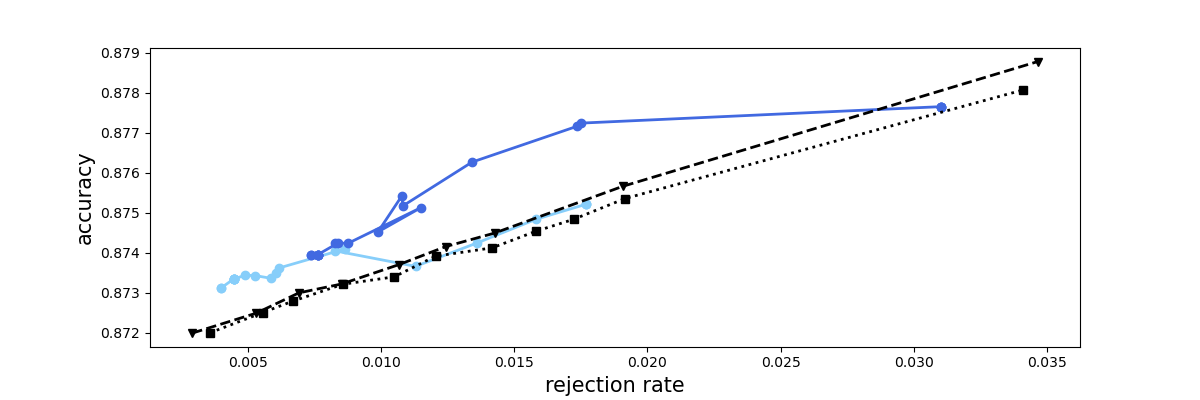
\includegraphics[width = \textwidth, trim={30 0 30 35}, clip]{arc_dries.png}
    \caption{Example of an accuracy-reject curve in which \citet{VanderPlas2023} compare two of their proposed models with a \changed{novelty} reject option (blue) with two models that were used as baseline (black). The proposed models outperform the baselines but the light blue model only does for rejection rates lower than $0.01$.}
    \label{fig:arc_metric}
\end{figure}

To assess the performance-rejection trade-off, a common approach is to evaluate the prediction quality (for non-rejected examples) by varying the rejection rate from $0\%$ to $100\%$, which is known as the \gls{arc}~\citep{Nadeem2010a}. This involves plotting the rejection rate on the x-axis and the prediction quality (e.g., accuracy) on the y-axis~\citep{Hanczar2014}. Higher curves indicate better performance. Alternatively, risk-based metrics like mean squared error can be plotted, with lower curves indicating better performance~\citep{SambuSeo2000}. Sometimes the predictor's performance on the rejected examples is also shown with the intuition that it should be worse on this subset of the data than on the accepted ones~\citep{Zou2011,Condessa2015,Condessa2015b}. 


When comparing two models using the \gls{arc} method, two scenarios arise. First, one model clearly outperforms the other in terms of prediction quality for all rejection rates. Second, the models show varying prediction quality across different rejection rates. To illustrate this, consider Figure~\ref{fig:arc_metric} where the light blue curve  only outperforms the black curves if the rejection rate is lower than $0.01$. When it is not clear which model performs best, the overall performance can be assessed using the \gls{aurc}, similar to the AUC in standard machine learning~\citep{Vanderlooy2006a,Vanderlooy2006,Landgrebe2006}. In this example, the \gls{aurc} of the light blue curve will be higher than the \gls{aurc} of the black curves, indicating that it performs better overall than the black curves.

\paragraph{Pros and Cons.} The main advantage of this category is that any prediction quality metric can be used on the y-axis. Moreover, they provide a high-level overview of how the model works for different rejection rates. However, generating these curves can be challenging for two reasons. 
First, some rejectors do not allow directly setting the rejection rate~\citep{Wu2007,Homenda2014}, but they might have other hyperparameters (e.g., rejection threshold). 
Mapping these to rejection rates may be challenging and may not be possible to achieve all possible rejection rates.
Second, altering the rejection rate of a model with rejection can require completely retraining the whole model. This may be too computationally demanding to perform a fine-grained analysis~\citep{Condessa2017}.


\subsection{Evaluating models through a cost function.}
\label{sec:eval_arc}
For classification tasks, one can ask the user to specify the costs for (mis)predictions as well as for rejection and evaluate a model by its (expected) total cost at test time.
Although the costs can be designed as a continuous function of the examples~\citep{Mozannar2020,De2021}, the cost function typically accounts only for three constant costs: the cost of correct prediction $C_c$, the cost of a prediction error $C_e$, and the cost of rejection $C_r$ such that $C_c < C_r < C_e$~\citep{DeStefano2000,Balsubramani2016,Condessa2013}. \changed{Without loss of generality, usually one assumes normalized costs, i.e., $C_c = 0$, $C_e = 1$ and $C_r\in [0,1]$ in which the normalized value for $C_r$ can be obtained from the initial values as $\frac{C_r - C_c}{C_e - C_c}$.} Although the costs need to be set based on some domain knowledge, there are two constraints for setting the rejection cost properly. First, it must be lower than a random predictor's average cost for a classification task with $K$ classes, i.e. $C_r \le \frac{1}{K}$~\citep{Cordella1995a,Herbei2006c}. Otherwise, the expected cost of always making a random prediction would be lower than the rejection cost, which nullifies the task of rejection. Second, one should account for possible imbalance classes by setting $C_r \le 1 - \max_{k \le K} P(Y = k)$, where $P(Y = k)$ is the class frequency~\citep{Perini2023}. In fact, for higher $C_r$, a naive model that always predicts the most frequent class $\bar{k}$ would obtain a cost equal to $1 - P(Y = \bar{k})$ and rejecting examples would not be worth it for higher rejection costs.

\paragraph{Pros and Cons.} The main benefit of this category is its high interpretability: given a final cost, we can easily go back to the causes that yield such a cost. Moreover, one can use the same cost function to optimize the model parameters during the learning phase. This ensures coherence between learning the optimal model at training time and measuring its performance at test time. However, this category has the key drawback that the user must set the cost function based on domain knowledge, which is not always easy to obtain. Setting different costs changes the quality of the models, which may end up ranking several compared models differently.
A way to alleviate this would be to make the Cost-Reject plot~\citep{Hanczar2019}, where, similar to the ARC, the x-axis and y-axis represent respectively the normalized rejection cost and the normalized prediction cost~\citep{Friedel2006,Abbas2019}.
